\documentclass[12pt,a4]{article}

\usepackage{mathptmx}
\usepackage{parskip}
\usepackage{graphicx}
\usepackage[estonian .notilde]{babel}
\usepackage{amssymb}
\usepackage[makeroom]{cancel}
\usepackage{amsmath}
\usepackage{braket}
\usepackage{setspace}
\onehalfspacing
\RequirePackage[utf8]{inputenc}
\RequirePackage[T1]{fontenc}
\RequirePackage[hidelinks]{hyperref}
\sloppy
\relpenalty=10000
\binoppenalty=10000
\usepackage{geometry}
\geometry{
	a4paper,
	total={160mm,235mm},
	left=25mm,
	top=20mm,
}
\usepackage{rotating}
\usepackage{systeme}
\usepackage{mathtools}
\usepackage{tikz}
\usepackage{pgfplots}
\newcommand{\mathcolorbox}[2]{\colorbox{#1}{$\displaystyle #2$}}
\usepackage{xcolor}
\usepackage{soul}
\usepackage{caption}
\usepackage{subcaption}

\begin{document}

\begin{figure}[!ht]
	\begin{subfigure}[b]{0.3\textwidth}
		\centering
		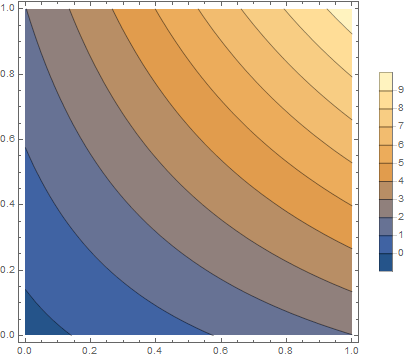
\includegraphics[width=\textwidth]{Joonised/PhiMu11Mu22I}
		\caption{$ \mu_{12} > |\nu_{12}| $}
	\end{subfigure}
	\hfill
	\begin{subfigure}[b]{0.3\textwidth}
		\centering
		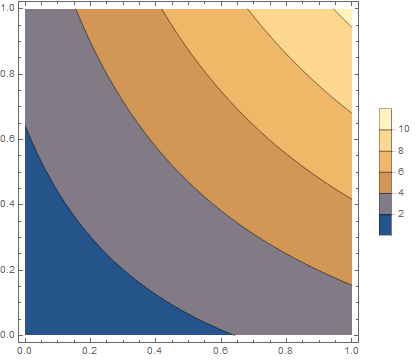
\includegraphics[width=\textwidth]{Joonised/PhiMu11Mu22II}
		\caption{$ \mu_{12} \sim | \nu_{12}| $}
	\end{subfigure}
	\hfill
	\begin{subfigure}[b]{0.3\textwidth}
		\centering
		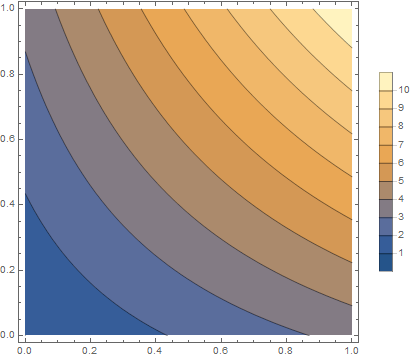
\includegraphics[width=\textwidth]{Joonised/PhiMu11Mu22III}
		\caption{$ \mu_{12} < | \nu_{12}| $}
	\end{subfigure}
	\caption{$ \Phi = \Phi (\mu_{11}, \mu_{22}, \mu_{12} = const) $}
\end{figure}
\begin{figure}[!ht]
	\centering
	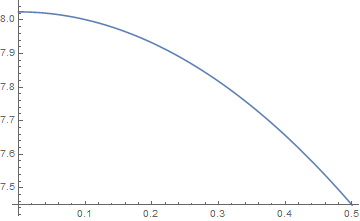
\includegraphics[width=0.3\textwidth]{Joonised/PhiMu12}
	\caption{$ \Phi = \Phi (\mu_{11} = const, \mu_{22} = const, \mu_{12}) $}
\end{figure}
\begin{figure}[!ht]
	\begin{subfigure}[b]{0.3\textwidth}
		\centering
		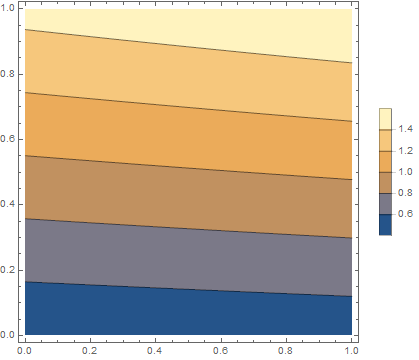
\includegraphics[width=\textwidth]{Joonised/Theta11Mu11Mu22I}
		\caption{$ \mu_{12} > |\nu_{12}| $}
	\end{subfigure}
	\hfill
	\begin{subfigure}[b]{0.3\textwidth}
		\centering
		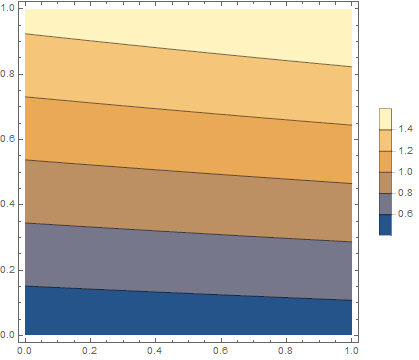
\includegraphics[width=\textwidth]{Joonised/Theta11Mu11Mu22II}
		\caption{$ \mu_{12} \sim | \nu_{12}| $}
	\end{subfigure}
	\hfill
	\begin{subfigure}[b]{0.3\textwidth}
		\centering
		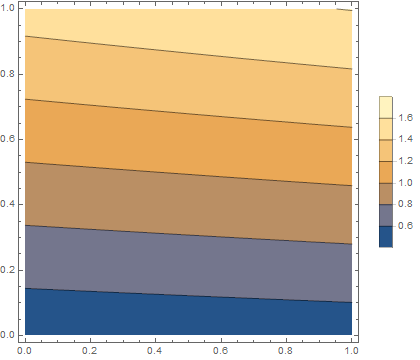
\includegraphics[width=\textwidth]{Joonised/Theta11Mu11Mu22III}
		\caption{$ \mu_{12} < | \nu_{12}| $}
	\end{subfigure}
	\caption{$ \Theta_{11} = \Theta_{11} (\mu_{11}, \mu_{22}, \mu_{12} = const, \nu_{11} = const) $}
\end{figure}
\begin{figure}[!ht]
	\centering
	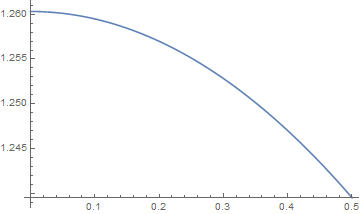
\includegraphics[width=0.3\textwidth]{Joonised/Theta11Mu12}
	\caption{$ \Theta_{11} = \Theta_{11} (\mu_{11} = const, \mu_{22} = const, \mu_{12}, \nu_{11} = const) $}
\end{figure}
\begin{figure}[!ht]
	\centering
	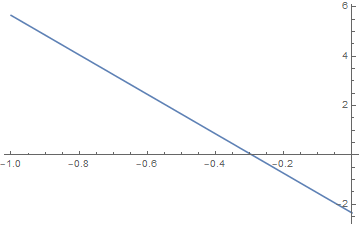
\includegraphics[width=0.3\textwidth]{Joonised/Theta11Nu11I}
	\caption{$ \Theta_{11} = \Theta_{11} (\mu_{11} = const, \mu_{22} = const, \mu_{12} = const, \nu_{11}) $}
\end{figure}
\begin{figure}[!ht]
	\begin{subfigure}[b]{0.3\textwidth}
		\centering
		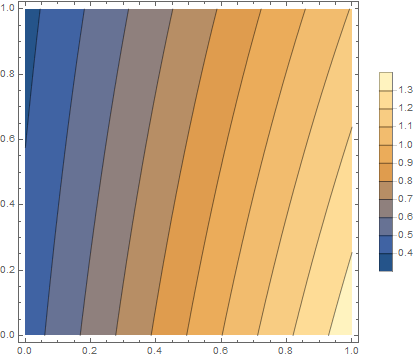
\includegraphics[width=\textwidth]{Joonised/Theta22Mu11Mu22I}
		\caption{$ \mu_{12} > |\nu_{12}| $}
	\end{subfigure}
	\hfill
	\begin{subfigure}[b]{0.3\textwidth}
		\centering
		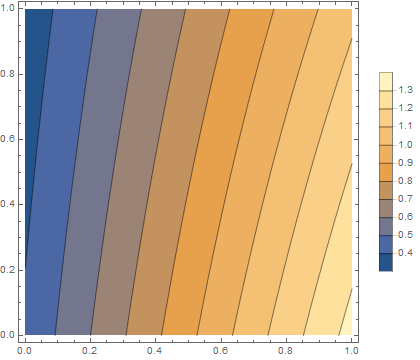
\includegraphics[width=\textwidth]{Joonised/Theta22Mu11Mu22II}
		\caption{$ \mu_{12} \sim | \nu_{12}| $}
	\end{subfigure}
	\hfill
	\begin{subfigure}[b]{0.3\textwidth}
		\centering
		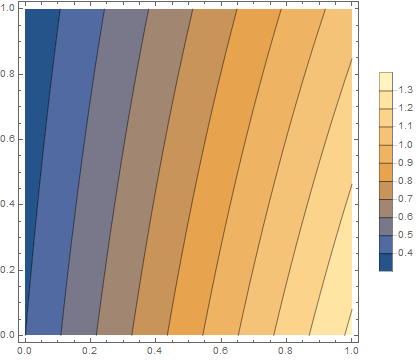
\includegraphics[width=\textwidth]{Joonised/Theta22Mu11Mu22III}
		\caption{$ \mu_{12} < | \nu_{12}| $}
	\end{subfigure}
	\caption{$ \Theta_{11} = \Theta_{11} (\mu_{11}, \mu_{22}, \mu_{12} = const, \nu_{11} = const) $}
\end{figure}
\begin{figure}[!ht]
	\centering
	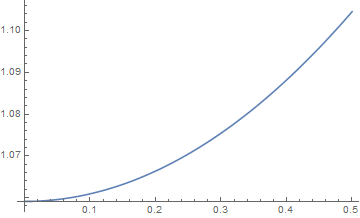
\includegraphics[width=0.3\textwidth]{Joonised/Theta22Mu12}
	\caption{$ \Theta_{22} = \Theta_{22} (\mu_{11} = const, \mu_{22} = const, \mu_{12}, \nu_{22} = const) $}
\end{figure}
\begin{figure}[!ht]
	\centering
	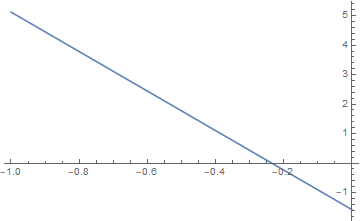
\includegraphics[width=0.3\textwidth]{Joonised/Theta22Nu22I}
	\caption{$ \Theta_{22} = \Theta_{22} (\mu_{11} = const, \mu_{22} = const, \mu_{12} = const, \nu_{22}) $}
\end{figure}
\begin{figure}[!ht]
	\begin{subfigure}[b]{0.3\textwidth}
		\centering
		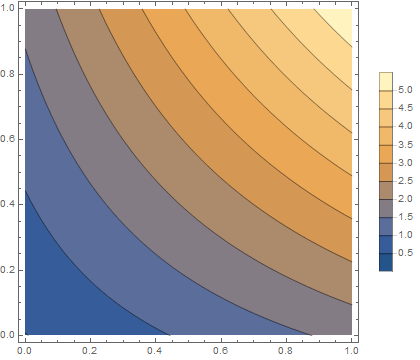
\includegraphics[width=\textwidth]{Joonised/ThetaMu11Mu22I}
		\caption{$ \mu_{12} > |\nu_{12}| $}
	\end{subfigure}
	\hfill
	\begin{subfigure}[b]{0.3\textwidth}
		\centering
		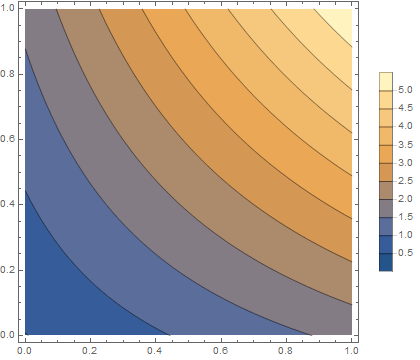
\includegraphics[width=\textwidth]{Joonised/ThetaMu11Mu22II}
		\caption{$ \mu_{12} \sim | \nu_{12}| $}
	\end{subfigure}
	\hfill
	\begin{subfigure}[b]{0.3\textwidth}
		\centering
		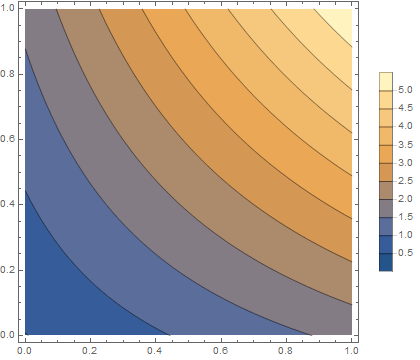
\includegraphics[width=\textwidth]{Joonised/ThetaMu11Mu22III}
		\caption{$ \mu_{12} < | \nu_{12}| $}
	\end{subfigure}
	\caption{$ \Theta = \Theta (\mu_{11}, \mu_{22}, \mu_{12} = const, \nu_{12} = const) $}
\end{figure}
\begin{figure}[!ht]
	\centering
	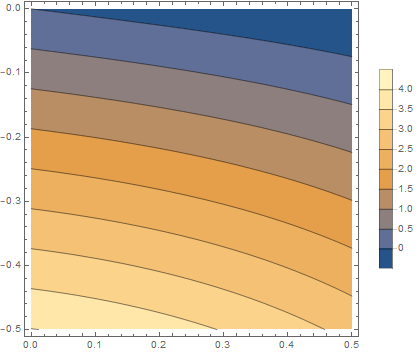
\includegraphics[width=0.3\textwidth]{Joonised/ThetaMu12Nu12}
	\caption{$ \Theta = \Theta (\mu_{11} = const, \mu_{22} = const, \mu_{12}, \nu_{12}) $}
\end{figure}
\begin{figure}[!ht]
	\begin{subfigure}[b]{0.3\textwidth}
		\centering
		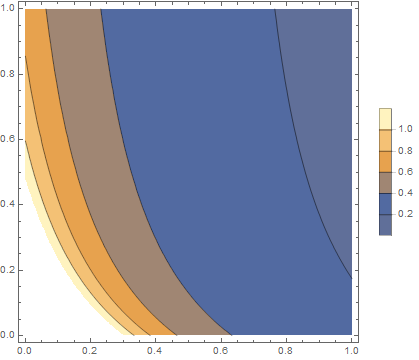
\includegraphics[width=\textwidth]{Joonised/Gamma11Mu11Mu22I}
		\caption{$ \mu_{12} > |\nu_{12}| $}
	\end{subfigure}
	\hfill
	\begin{subfigure}[b]{0.3\textwidth}
		\centering
		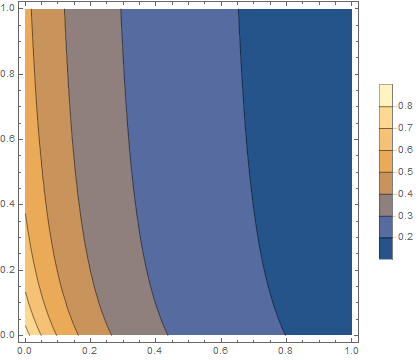
\includegraphics[width=\textwidth]{Joonised/Gamma11Mu11Mu22II}
		\caption{$ \mu_{12} \sim | \nu_{12}| $}
	\end{subfigure}
	\hfill
	\begin{subfigure}[b]{0.3\textwidth}
		\centering
		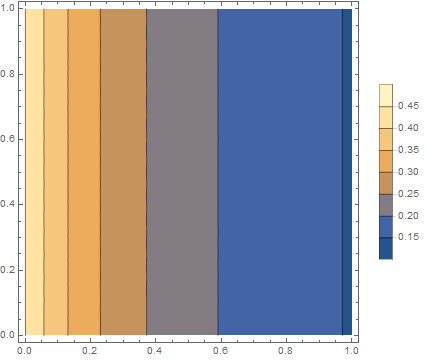
\includegraphics[width=\textwidth]{Joonised/Gamma11Mu11Mu22III}
		\caption{$ \mu_{12} < | \nu_{12}| $}
	\end{subfigure}
	\caption{$ \Gamma_{11} = \Gamma_{11} (\mu_{11}, \mu_{22}, \mu_{12} = const, \nu_{11} = const) $}
\end{figure}
\begin{figure}[!ht]
	\centering
	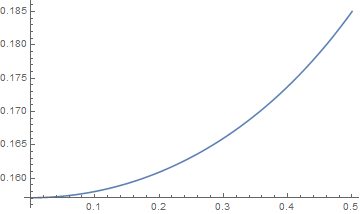
\includegraphics[width=0.3\textwidth]{Joonised/Gamma11Mu12}
	\caption{$ \Gamma_{11} = \Gamma_{11} (\mu_{11} = const, \mu_{22} = const, \mu_{12}, \nu_{11} = const) $}
\end{figure}
\begin{figure}[!ht]
	\centering
	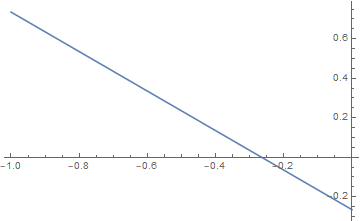
\includegraphics[width=0.3\textwidth]{Joonised/Gamma11Nu11I}
	\caption{$ \Gamma_{11} = \Gamma_{11} (\mu_{11} = const, \mu_{22} = const, \mu_{12} = const, \nu_{11}) $}
\end{figure}
\begin{figure}[!ht]
	\begin{subfigure}[b]{0.3\textwidth}
		\centering
		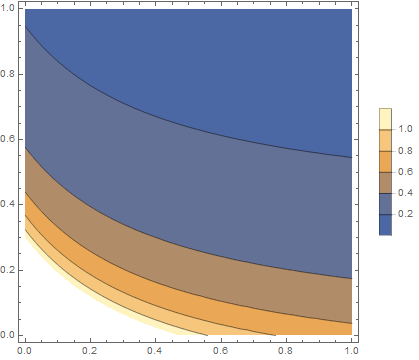
\includegraphics[width=\textwidth]{Joonised/Gamma22Mu11Mu22I}
		\caption{$ \mu_{12} > |\nu_{12}| $}
	\end{subfigure}
	\hfill
	\begin{subfigure}[b]{0.3\textwidth}
		\centering
		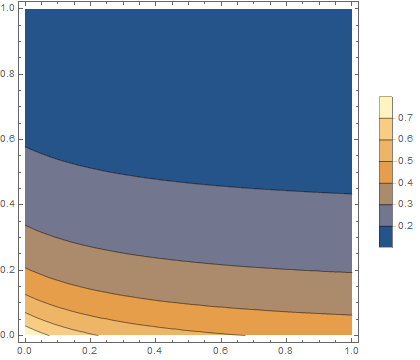
\includegraphics[width=\textwidth]{Joonised/Gamma22Mu11Mu22II}
		\caption{$ \mu_{12} \sim | \nu_{12}| $}
	\end{subfigure}
	\hfill
	\begin{subfigure}[b]{0.3\textwidth}
		\centering
		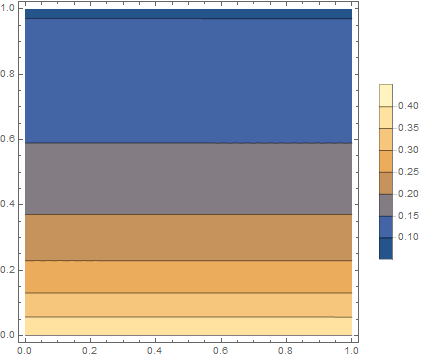
\includegraphics[width=\textwidth]{Joonised/Gamma22Mu11Mu22III}
		\caption{$ \mu_{12} < | \nu_{12}| $}
	\end{subfigure}
	\caption{$ \Gamma_{11} = \Gamma_{11} (\mu_{11}, \mu_{22}, \mu_{12} = const, \nu_{11} = const) $}
\end{figure}
\begin{figure}[!ht]
	\centering
	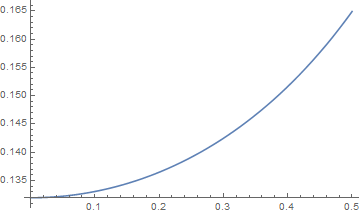
\includegraphics[width=0.3\textwidth]{Joonised/Gamma22Mu12}
	\caption{$ \Gamma_{22} = \Gamma_{22} (\mu_{11} = const, \mu_{22} = const, \mu_{12}, \nu_{22} = const) $}
\end{figure}
\begin{figure}[!ht]
	\centering
	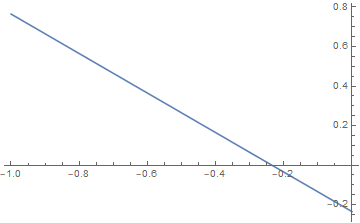
\includegraphics[width=0.3\textwidth]{Joonised/Gamma22Nu22I}
	\caption{$ \Gamma_{22} = \Gamma_{22} (\mu_{11} = const, \mu_{22} = const, \mu_{12} = const, \nu_{22}) $}
\end{figure}
\begin{figure}[!ht]
	\begin{subfigure}[b]{0.3\textwidth}
		\centering
		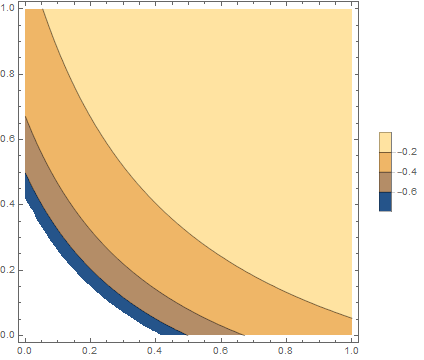
\includegraphics[width=\textwidth]{Joonised/GammaMu11Mu22I}
		\caption{$ \mu_{12} > |\nu_{12}| $}
	\end{subfigure}
	\hfill
	\begin{subfigure}[b]{0.3\textwidth}
		\centering
		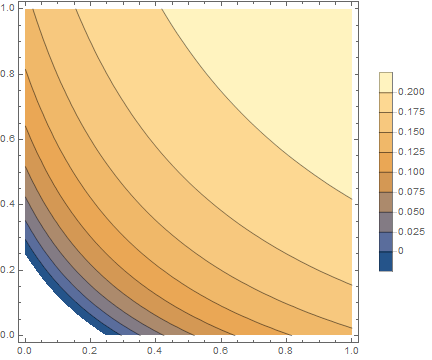
\includegraphics[width=\textwidth]{Joonised/GammaMu11Mu22II}
		\caption{$ \mu_{12} \sim | \nu_{12}| $}
	\end{subfigure}
	\hfill
	\begin{subfigure}[b]{0.3\textwidth}
		\centering
		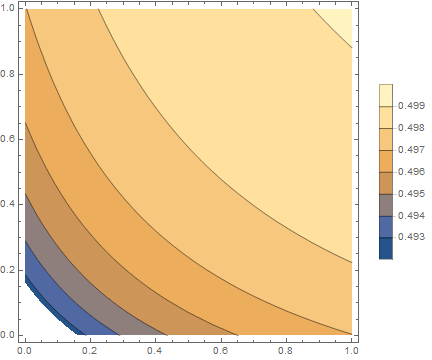
\includegraphics[width=\textwidth]{Joonised/GammaMu11Mu22III}
		\caption{$ \mu_{12} < | \nu_{12}| $}
	\end{subfigure}
	\caption{$ \Gamma = \Gamma (\mu_{11}, \mu_{22}, \mu_{12} = const, \nu_{12} = const) $}
\end{figure}
\begin{figure}[!ht]
	\centering
	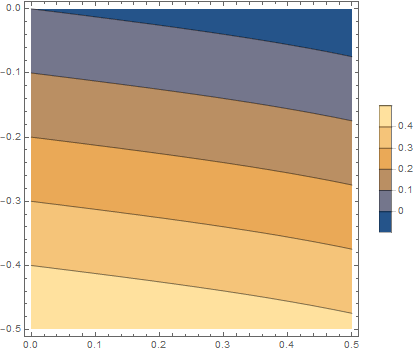
\includegraphics[width=0.3\textwidth]{Joonised/GammaMu12Nu12}
	\caption{$ \Gamma = \Gamma (\mu_{11} = const, \mu_{22} = const, \mu_{12}, \nu_{12}) $}
\end{figure}

\end{document}